\chapter{Testovi i ispiti 2018/2019}

\section{Programiranje 2, kolokvijum, april 2019.}
\subsection{Grupa I}

\begin{enumerate}
\item Kao argument komandne linije zadaje se broj $k$ ($k \ge 0$).  Napisati program koji sa
standardnog ulaza učitava niz celih brojeva sve do kraja ulaza (EOF). Osim da
je minimalna dimenzija niza jednaka $1$, ne praviti dodatne pretpostavke o
dimenziji. Rotirati elemente niza za $k$ mesta i ispisati novodobijeni niz.

U slučaju greške na standardni izlaz za greške ispisati -1. \\
\emph{Uputstvo}: Koristiti funkciju za realokaciju memorije sa korakom 10. Dozvoljeno je korišćenje pomoćnog niza.
\begin{verbatim}
Primer 1:            Primer 2:             Primer 3:         Primer 4:
./a.out 2            ./a.out 5             ./a.out  -3       ./a.out 4 
1 2 3 4 5 6 7        1 2 3                                   1 2 3 4 5 6 7 8 9 10

6 7 1 2 3 4 5        2 3 1                 -1                7 8 9 10 1 2 3 4 5 6
\end{verbatim}


\item U datoteci čije se ime zadaje kao prvi argument komandne linije nalaze se
podaci o knjigama u biblioteci. U svakom redu datoteke nalazi se naziv knjige,
ime, prezime autora, žanr i broj primeraka. Pretpostaviti da je maksimalna
dužina reda u datoteci $200$ karaktera. Kao drugi argument komandne linije
zadaje se žanr. Napisati program koji na standardni izlaz ispisuje sve knjige
(naziv knige, ime i prezime autora, žanr i broj primeraka) koje su iz datog
žanra. U slučaju greške na standardni izlaz za greške ispisati -1.
\begin{verbatim}
Primer 1:                                              Primer 2:
./a.out dat.txt -roman                                 ./a.out knjige.txt -satira

dat.txt:                                               knjige.txt:
Stranac, Alber Kami, roman, 3                          Stranac, Alber Kami, roman, 3
Hamlet, Viljam Šekspir, tragedija, 5                   Hamlet, Viljam Šekspir, tragedija, 5
Mrtve duše, Nikolaj Gogoglj, satira, 2                 Mrtve duše, Nikolaj Gogoglj, satira, 2
Proces, Franc Kafka, roman, 1                          Proces, Franc Kafka, roman, 1
Dnevnik Ane Frank, Ana Frank, dnevnik, 3               Dnevnik Ane Frank, Ana Frank, dnevnik, 3
Don Kihot, Migel de Servantes, satira, 5               Don Kihot, Migel de Servantes, satira, 5
Dekameron, Đovani Bokačo, novela, 3                    Dekameron, Đovani Bokačo, novela, 3
Jadnici, Viktor Igo, roman, 1                          Jadnici, Viktor Igo, roman, 1
                                                   

Stranac, Alber Kami, roman, 3                          Mrtve duše, Nikolaj Gogoglj, satira, 2
Proces, Franc Kafka, roman, 1                          Don Kihot, Migel de Servantes, satira, 5
Jadnici, Viktor Igo, roman, 1
--------------------------------------------------------------------------------------------------

Primer 3:                                              Primer 4:
./a.out biblioteka.txt -poezija                        ./a.out dat.txt

biblioteka.txt:
Stranac, Alber Kami, roman, 3                          -1
Hamlet, Viljam Šekspir, tragedija, 5
Mrtve duše, Nikolaj Gogoglj, satira, 2
Proces, Franc Kafka, roman, 1
Dnevnik Ane Frank, Ana Frank, dnevnik, 3
Don Kihot, Migel de Servantes, satira, 5
Dekameron, Đovani Bokačo, novela, 3
Jadnici, Viktor Igo, roman, 1
\end{verbatim}

\item Napisati rekurzivnu funkciju {\tt int f3(int x)} koja u datom broju $x$ 
računa broj cifara koje su manje od svog levog suseda. Napisati potom program
koji testira ovu funkciju za vrednost koja se zadaje sa standardnog ulaza.
{\bf Napomena: Nije dozvoljeno kori\v s\'cenje stati\v ckih ili globalnih
promenljivih ili menjanje potpisa funkcije.}
\begin{verbatim}
Primer 1:        Primer 2:        Primer 3:      Primer 4:
25151            3                -67432         8888

2                0                3              0
\end{verbatim}

\end{enumerate}

\subsection{Grupa II}

\begin{enumerate} 
\item Argumenti komandne linije zadaju se $2$ broja -- dimenzija niza $n$ ($n \ge 1$)
i broj $k$ ($k \ge 1$). Sa standarnog ulaza u\v citava se niz  celih brojeva
dimenzije $n$. Ispisati $k$ slu\v cajno izabranih brojeva iz niza. Kao
parametar ({\em seed}) za funkciju {\tt random} postaviti $5$. U slu\v
caju gre\v ske na standarni izlaz za gre\v ske ispisati -1.
\begin{verbatim}
Primer 1:          Primer 2:                                Primer 3:       Primer 4:
./a.out 4 2        ./a.out 12 3                             ./a.out 5       ./a.out 6 1
3 -90 8 16         9 100 200 3 -88 -93 43 7 6 8 23 90                       1 15 -10 78 200 -64

16 -90             7 -93 43                                 -1              15        
\end{verbatim}

\item Ime datoteke se zadaje kao argument komandne linije. Za svaku liniju u
datoteci ispisati broj linije, dve ta\v cke i ukupan broj cifara koji se u toj
liniji pojavljuju. U slu\v caju gre\v ske na standarni izlaz za gre\v ske
ispisati -1. Linije u datoteci se broje po\v cev\v si od $1$. Maksimalna du\v
zina linije je $200$ karaktera.
\begin{verbatim}
Primer 1:                    Primer 2:                         Primer 3:
./a.out dat.txt              ./a.out statistika.txt            ./a.out 

dat.txt:                     statistika.txt:                   -1
Zabavno je uciti             2018/2019:
programiranje2!!!            broj studenta i smera: 246
1: 0                         broj studenata r smera: 90
2: 1                         broj studenata l smera: 22

                             1: 8
                             2: 3
                             3: 2
                             4: 2

-------------------------------------------------------------------------------------------

Primer 4:
./a.out zadaci.txt

zadaci.txt:
zad1. uneti brojeve
zad2. broj 23 je
napomena.                             

1: 1
2: 3
3: 0
\end{verbatim}

\item  Napisati rekurzivnu funkciju {\tt int zbir(int x)} koja računa zbir
cifara u heksadekadnom zapisu datog neoznačenog celog broja. Napisati potom
program koji testira ovu funkciju za vrednost koja se zadaje sa standardnog
ulaza u heksadekadnom formatu.  {\bf Napomena: Nije dozvoljeno kori\v s\'cenje
stati\v ckih ili globalnih promenljivih ili menjanje potpisa funkcije.}
\begin{verbatim}
Primer 1:            Primer 2:          Primer 3:        Primer 4:
0xFA1                0x111              0x7A             0xB
 
26                   3                  30               11
\end{verbatim} 

\end{enumerate}

\section{Programiranje 2, ispit, jun1 2019.}
\subsection{Grupa I}

\begin{enumerate} 
\item U datoteci se nalaze podaci o transakcijama korisnika po karticama. Korisnik može imati više 
      kartica zadatih sa brojem koji ima $16$ cifara. U svakom redu datoteke se nalazi broj kartice,
      a potom realan broj koji označava iznos. Pozitivan iznos označava uplatu, a negativan iznos isplatu sa računa.
      Kao argumente komadne linije korisnik zadaje ime i prezime i opciju. Otvoriti datoteku čiji je naziv {\tt ime\_prezime.txt}
      (zameniti ime, prezime sa onim što je uneo korisnik) i odrediti saldo za svaku karticu (ukupnu sumu svih uplata i isplata).
      Ukoliko je korisnik zadao opciju {\tt -kartica} sortirati podatke prema broju kartice i ispisati na standardni izlaz.
      Ukoliko je korisnik zadao opciju {\tt -suma} sortirati opadajuće prema sumi na karticama i isipisati na standardni izlaz.
      Ne praviti nikakve pretpostavke o ukupnom broju transakcija, koristiti funkciju za realokaciju memorije sa korakom $10$. 
      U slučaju greške ispisati $-1$ na standradni izlaz za greške. Pretpostaviti da su brojevi kartica ispravno zadati i ne 
      proveravati njihovu ispravnost.

\begin{verbatim}
Primer 1:                                             Primer 2:

Pozivanje: ./a.out Marko Markovic -kartica            Pozivanje: ./a.out Marko Markovic -suma
Datoteka Marko_Markovic.txt:                          Datoteka Marko_Markovic.txt:
1245678915261782    500                               1245678915261782    500
9081972619261617    1000                              9081972619261617    1000
1245678915261782    -200                              1245678915261782    -200
9181009191010236    -400.89                           9181009191010236    -400.89
9181009191010236    2002.99                           9181009191010236    2002.99
9081972619261617    56789.74                          9081972619261617    56789.74
1245678915261782    300.99                            1245678915261782    300.99
1245678915261782    7816.25                           1245678915261782    7816.25
9081972619261617    -5006.12                          9081972619261617    -5006.12
4890019103002038    13.3                              4890019103002038    13.3         

Standarni izlaz:                                      Standarni izlaz:
1245678915261782 8417.240000                          9081972619261617 52783.620000
4890019103002038 13.300000                            1245678915261782 8417.240000
9081972619261617 52783.620000                         9181009191010236 1602.100000
9181009191010236 1602.100000                          4890019103002038 13.300000
---------------------------------------------------------------------------------------------------

Primer 3:                                             Primer 4:
Pozivanje: ./a.out Janko Jankovic -novac              Pozivanje: ./a.out Jelena Protic -suma
                                                      Datoteka Jelena_Protic.txt:
Datoteka Janko_Jankovic.txt ne postoji                1818228384779393  230.15
                                                      9876798273829376  220
                                                      9876798273829376  10.30
Standardni izlaz za greske:
-1                                                    Standardni izlaz:
                                                      9876798273829376 230.300000
                                                      1818228384779393 230.150000
\end{verbatim}

\item Napisati funkciju \texttt{unsigned zameni(unsigned x)} koja zamenjuje prva dva bajta sa druga dva bajta, a druga dva bajta sa prva dva bajta broja \texttt{x} (a ostali bitovi ostaju nepromenjeni, bajtovi se broje sa desna na levo). Ispisati tako transformisan broj na standardni izlaz.

\begin{verbatim}
Primer 1:             Primer 2:                Primer 3:               Primer 4:

Standardni ulaz:      Standardni ulaz:         Standardni ulaz:        Standardni ulaz:
0xffffaaaa            0x0                      0xff0055                0x7f

Standardni izlaz:     Standardni izlaz:        Standardni izlaz:       Standardni izlaz:
0xaaaaffff            0x0                      0x5500ff                0x7f0000
\end{verbatim}    
   

\item Sa standarnog ulaza unosi se lista celih brojeva. Izmeniti listu tako da između 
      svaka dva parna broja u listi umeće nulu. Ispisati dobijenu listu na standardni izlaz. 
      {\em Napomena: Za rad sa listama obavezno koristiti datu biblioteku 
      ({\tt liste.c} i {\tt liste.h}). Zadatak se mora rešiti korišćenjem listi i 
      uneta lista mora biti zaista modifikovana. U suprotnom broj osvojenih poena je $0$.}
\begin{verbatim}
Primer 1:                                     Primer 2:                

Standardni ulaz:                              Standardni ulaz:         
20 10 7 17 16 -30 1                           5                        

Standardni izlaz:                             Standardni izlaz:        
[20, 0, 10, 7, 17, 16, 0, -30, 1]             [5]                      
--------------------------------------------------------------------

Primer 3:                                     Primer 4:

Standardni ulaz:                              Standardni ulaz:
9 10 8 200 400 500                            1 2 3

Standardni izlaz:                             Standardni izlaz:
[9, 10, 0, 8, 0, 200, 0, 400, 0, 500]         [1, 2, 3]
\end{verbatim}  

\item Sa standardnog ulaza se učitavaju elementi binarnog pretraživačkog (tj. binarnog uređenog) stabla koji su celi brojevi, sve do kraja ulaza 
(\texttt{EOF}). Prvo formirati stablo od unetih brojeva, a zatim ispisati na standardni izlaz one vrednosti čvorova stabla čija je vrednost jednaka zbiru vrednosti njegovih neposrednih potomaka, pri čemu ako čvor nema nekog potomka njegov doprinos vrednosti zbira je 0. Listovi nemaju nijednog potomka, što znači da se njihova vrednost ispisuje isključivo ukoliko je jednaka 0. Tražene vrednosti ispisati u onom redosledu koji se dobija \textbf{infiksnim obilaskom stabla} (sleva nadesno). U slučaju greške ispisati -1 na standardni izlaz za greške. \textit{Napomena: Za rad sa binarnim pretraživačkim stablima obavezno koristiti datu biblioteku (\textbf{stabla.h} i \textbf{stabla.c}). Zadatak se mora rešiti korišćenjem binarnog pretraživačkog stabla i ispis traženih vrednosti mora biti izvršen obilaskom čvorova stabla. U suprotnom broj osvojenih poena je $0$.}

\begin{verbatim}
        -5                     4                       1                       1    
        / \                   / \                     /                       / \
      -5   0                 2   7                   1                      -3   4
      /   / \               /   / \                 /                       /   
    -8   0   3             1   7   9               1                      -3   
                              /                   /                       / \
                             6                   1                      -3   0

Primer 1:               Primer 2:               Primer 3:               Primer 4:                

Standardni ulaz:        Standardni ulaz:        Standardni ulaz:        Standardni ulaz: 
-5 -5 0 0 3 -8          4 2 1 7 7 9 6           1 1 1 1                 1 4 -3 -3 -3 0

Standardni izlaz:       Standardni izlaz:       Standardni izlaz:       Standardni izlaz:        
-5 0                                            1 1 1                   -3 -3 0 1 
\end{verbatim}  

\end{enumerate}

\subsection{Grupa II}

\begin{enumerate} 
\item Na takmičenju u programiranju učesnici se rangiraju u odnosu na vreme izvršavanja njihovih programa. U datoteci čije se ime zadaje kao argument komandne linije dati su nazivi izvršnih fajlova i vremena njihovog izvršavanja u formatu \texttt{hh:mm:ss.sss} (\texttt{hh}-broj sati, \texttt{mm}-broj minuta, \texttt{ss}-broj sekundi i \texttt{sss}-broj milisekundi). Potrebno je napraviti konačnu rang listu kandidata. Napisati program koji čita podatke o izvršnim fajlovima iz date datoteke, sortira ih rastuće u odnosu na vreme izvršavanja i ispisuje konačnu rang listu na standardni izlaz. Pretpostaviti da su nazivi izvršnih fajlova maksimalne dužine $50$ karaktera. 
Ne praviti nikakve pretpostavke o ukupnom broju izvršnih fajlova, 
koristiti funkciju za realokaciju memorije sa korakom $10$.  
U slučaju greške ispisati -1 na standardni izlaz za greške.

\begin{verbatim}
Primer 1:                         Primer 2:                           Primer 3:

Pozivanje: ./a.out dat.txt        Pozivanje: ./a.out rez.txt        Pozivanje: ./a.out tmp.txt

Datoteka dat.txt:                 Datoteka rez.txt:                 Datoteka tmp.txt:
a.out 00:01:12.670                k011_izvrsni 00:02:00.670         rb092.out 01:02:00.472
prvi 00:01:09.401                 k020_izvrsni 00:02:09.001         rb119.out 00:56:06.021 
1.out 00:01:17.092                k007_izvrsni 00:02:17.002         rb002.out 00:59:04.010
tmp.out 00:01:19.607              k190_izvrsni 00:01:59.630         rb073.out 01:00:55.934       
izvrsni 00:01:03.342              k082_izvrsni 00:02:06.332         rb108.out 01:02:14.732
zavrsna_verzija 00:00:58:921      k113_izvrsni 00:01:58:947         rb033.out 00:58:27:375
1_1 00:01:00.738                  k056_izvrsni 00:02:01.767

Standarni izlaz:                  Standarni izlaz:                  Standardni izlaz:
zavrsna_verzija 0:0:58.921        k113_izvrsni 0:1:58.947           rb119.out 0:56:6.21
1_1 0:1:0.738                     k190_izvrsni 0:1:59.630           rb033.out 0:58:27.375
izvrsni 0:1:3.342                 k011_izvrsni 0:2:0.670            rb002.out 0:59:4.10
prvi 0:1:9.401                    k056_izvrsni 0:2:1.767            rb073.out 1:0:55.934
a.out 0:1:12.670                  k082_izvrsni 0:2:6.332            rb092.out 1:2:0.472
1.out 0:1:17.92                   k020_izvrsni 0:2:9.1              rb108.out 1:2:14.732
tmp.out 0:1:19.607                k007_izvrsni 0:2:17.2

----------------------------------------------------------------------------------------------

Primer 4:  
                                           
Pozivanje: ./a.out dat.txt              
                        
Datoteka dat.txt ne postoji
                            
Standardni izlaz za greske: 
-1                                                                                                                                        
\end{verbatim}

\item Napisati funkciju \texttt{unsigned invertuj(unsigned x)} koja invertuje bitove na neparnim pozicijama unutar prva dva bajta, a invertuje bitove na parnim pozicijama unutar druga dva bajta broja \texttt{x} (a ostali bitovi ostaju nepromenjeni, bajtovi se broje sa desna na levo). Ispisati tako transformisan broj na standardni izlaz.

\begin{verbatim}
Primer 1:             Primer 2:                Primer 3:               Primer 4:

Standardni ulaz:      Standardni ulaz:         Standardni ulaz:        Standardni ulaz:
0xffffffff            0x0                      0xff00ff                0x7a

Standardni izlaz:     Standardni izlaz:        Standardni izlaz:       Standardni izlaz:
0x5555aaaa            0xaaaa5555               0xaa5555aa              0xaaaa552f
\end{verbatim}  


\item Sa standardnog ulaza unose se elementi liste koji su celi brojevi, sve do kraja ulaza (\texttt{EOF}). Prvo formirati listu od unetih brojeva, a zatim ispisati na standardni izlaz vrednosti elementa liste čija je vrednost veća ili jednaka od vrednosti levog suseda. Prvi element liste nema levog suseda. U slučaju greške ispisati -1 na standardni izlaz za greške. \textit{Napomena: Za rad sa listama obavezno koristiti datu biblioteku (\textbf{liste.h} i \textbf{liste.c}). Zadatak se mora rešiti korišćenjem listi i ispis traženih vrednosti mora biti izvršen obilaskom elmenata liste. U suprotnom broj osvojenih poena je $0$.}

\begin{verbatim}
Primer 1:                Primer 2:                Primer 3:                Primer 4:        

Standardni ulaz:         Standardni ulaz:         Standardni ulaz:         Standardni ulaz:         
2 -3 4 7 12 5 0          -1 3 4 1 -3 2 2          1 1 1 1 1 1              15

Standardni izlaz:        Standardni izlaz:        Standardni izlaz:        Standardni izlaz:        
4 7 12                   3 4 2 2                  1 1 1 1 1
\end{verbatim}  

\item Sa standardnog ulaza se učitavaju elementi binarnog pretraživačkog stabla (binarnog uređenog stabla), 
      sve do kraja ulaza. Svaki čvor duplirati i umetnuti kao levo dete postojećeg čvora (pogledati primer ispod).
      \textit{Napomena: Za rad sa binarnim pretraživačkim stablima obavezno koristiti datu biblioteku (\textbf{stabla.h} i \textbf{stabla.c}). Zadatak se mora rešiti korišćenjem binarnog pretraživačkog stabla i ispis traženih vrednosti mora biti izvršen obilaskom čvorova stabla. U suprotnom broj osvojenih poena je $0$.}

\begin{verbatim}
         2                      2
        / \                    / \  
       1   3                  2   3
                             /   /
                            1    3 
                           /
                          1

Primer 1:               Primer 2:                

Standardni ulaz:        Standardni ulaz:         
2 1 3                   10 3 90 15 6 7 8 45 20 -1           

Standardni izlaz:       Standardni izlaz:        
1 1 2 2 3 3             -1 -1 3 3 6 6 7 7 8 8 10 10 15 15 20 20 45 45 90 90
---------------------------------------------------------------------------

Primer 3:               Primer 4:

Standardni ulaz:        Standardni ulaz:
5 3 4 10                8 -10 11

Standardni izlaz:       Standardni izlaz:
3 3 4 4 5 5 10 10       -10 -10 8 8 11 11         
\end{verbatim}  

\end{enumerate}

\section{Programiranje 2, ispit, jun2 2019.}

\begin{enumerate} 
\item Asistent je pregledao ispit i kako koji rad je pregledao beležio je u \texttt{.txt} fajlu ime, prezime, broj indeksa i broj osvojenih poena studenta. Pomoći asistentu da formira konačan spisak sa rezultatima sortiranim opadajuće u odnosu na broj poena. Ukoliko je broj poena isti sortirati prema prema prezimenu rastuće. Napisati program koji čita zabeležene rezultate ispita iz datoteke čije se ime zadaje kao argument komandne linije, a zatim ih sortira i ispisuje konačan spisak sa sortiranim rezultatima na standardni izlaz. Pretpostaviti da su imena i prezimena studenata maksimalne dužine $20$ karaktera. Nije poznat ukupan broj studenata u datoteci. U slučaju greške ispisati -1 na standardni izlaz za greške.

\begin{verbatim}
Primer 1:                         Primer 2:                           Primer 3:

Pozivanje: ./a.out dat.txt        Pozivanje: ./a.out rez.txt        Pozivanje: ./a.out tmp.txt

Datoteka dat.txt:                 Datoteka rez.txt:                 Datoteka tmp.txt:
Ana Markovic 18/2018 20           Filip Tomic 109/2018 18           Mila Petrovic 129/2018 15
Petar Stankovic 32/2018 14        Dunja Stanojevic 33/2018 22       Nikola Jovic 73/2018 23
Mirko Simic 211/2017 12           Sara Radojevic 271/2018 15        Stefan Tomic 54/2018 18
Marija Tirnanic 8/2018 24         Dusan Petrovic 9/2018  25         Tamara Panic 192/2016 3
Nikola Lazic 108/2018 19          Nemanja Terzic 187/2017 10        Dusan Maric 312/2017 14   
Sanja Jovanovic 319/2017 16       Stefan Nikolic 89/2018 15         Petar Stojic 5/2018 20
Milos Petrovic 231/2017 8         Tijana Gajic 230/2017 17
                                  Dimitrije Savic 221/2018 15            

Standarni izlaz:                  Standarni izlaz:                  Standardni izlaz:
Marija Tirnanic 8/2018 24         Dusan Petrovic 9/2018  25         Nikola Jovic 73/2018 23
Ana Markovic 18/2018 20           Dunja Stanojevic 33/2018 22       Petar Stojic 5/2018 20
Nikola Lazic 108/2018 19          Filip Tomic 109/2018 18           Stefan Tomic 54/2018 18
Sanja Jovanovic 319/2017 16       Tijana Gajic 230/2017 17          Mila Petrovic 129/2018 15
Petar Stankovic 32/2018 14        Stefan Nikolic 89/2018 15         Dusan Maric 312/2017 14 
Mirko Simic 211/2017 12           Sara Radojevic 271/2018 15        Tamara Panic 192/2016 3
Milos Petrovic 231/2017 8         Dimitrije Savic 221/2018 15
                                  Nemanja Terzic 187/2017 10
----------------------------------------------------------------------------------------------

Primer 4:  
                                           
Pozivanje: ./a.out dat.txt              
                        
Datoteka dat.txt ne postoji
                            
Standardni izlaz za greske: 
-1                                                                                                                                        
\end{verbatim}

\item Napisati funkciju \texttt{unsigned izmeni(unsigned x)} koja korišćenjem bitovskih operatora menja dati broj \texttt{x} tako da se u heksadekadnom zapisu na parnim pozicijama nalazi cifra \texttt{F}, dok cifre na neparnim pozicijama ostaju nepromenjene. Ispistati tako transformisan broj na standardni izlaz.

\begin{verbatim}
Primer 1:             Primer 2:               Primer 3:               Primer 4:

Standardni ulaz:      Standardni ulaz:        Standardni ulaz:        Standardni ulaz:
0x2B39                0x0                     0xAAAACCCC              0xFFFF

Standardni izlaz      Standardni izlaz:       Standardni izlaz:       Standardni izlaz:
0xf0f2f3f             0xf0f0f0f               0xafafcfcf              0xf0fffff
\end{verbatim} 

\item Sa standarnog ulaza unosi se lista celih brojeva. Datu listu podeliti na listu pozitivnih brojeva i listu negativnih brojeva
      (0 se smatra pozitivnim brojem). Prilikom podele liste nije dozvoljeno kreiranje novih čvorova. Ispisati dobijene liste na
      standardni izlaz. 
      {\em Napomena: Za rad sa listama obavezno koristiti datu biblioteku 
      ({\tt liste.c} i {\tt liste.h}). Zadatak se mora rešiti korišćenjem listi, u suprotnom broj osvojenih poena je $0$.
      Smatra se netačnim rešenje u kome se elementi liste samo ispisuju, a lista se pri tome ne menja.}
\begin{verbatim}
Primer 1:               Primer 2:             Primer 3:                   Primer 4:   

Standardni ulaz:        Standardni ulaz:      Standardni ulaz:            Standardni ulaz:
20 10 -7 17 0 -30 1     5                     -9 -10 8 -200 -400 500      -1 -2 -3

Standardni izlaz:       Standardni izlaz:     Standardni izlaz:           Standardni izlaz:
[20, 10, 17, 0, 1]      [5]                   [8, 500]                    []
[-7, -30]               []                    [-9, -10, -200, -400]       [-1, -2, -3]    
\end{verbatim}  

\item Sa standardnog ulaza se učitavaju elementi binarnog pretraživačkog (tj. binarnog uređenog) stabla koji su celi brojevi, sve do kraja ulaza (\texttt{EOF}). Prvo se unosi ceo broj $k$ ($k \ge 1$), a zatim i elementi stabla sve do kraja ulaza. Prvo formirati stablo od unetih brojeva, a zatim odrediti sumu po $k$-toj glavnoj dijagonali datog stabla (pogledati sliku u prilogu). Dijagonale se broje počevši od $1$. Rezultat ispisati na standardni izlaz.
\textit{Napomena: Za rad sa binarnim pretraživačkim stablima obavezno koristiti datu biblioteku (\textbf{stabla.h} i \textbf{stabla.c}). Zadatak se mora rešiti korišćenjem binarnog pretraživačkog stabla i ispis traženih vrednosti mora biti izvršen obilaskom čvorova stabla. U suprotnom broj osvojenih poena je $0$.}

\begin{figure}[h!]
    \centering
    \begin{minipage}[b]{0.50\textwidth}
        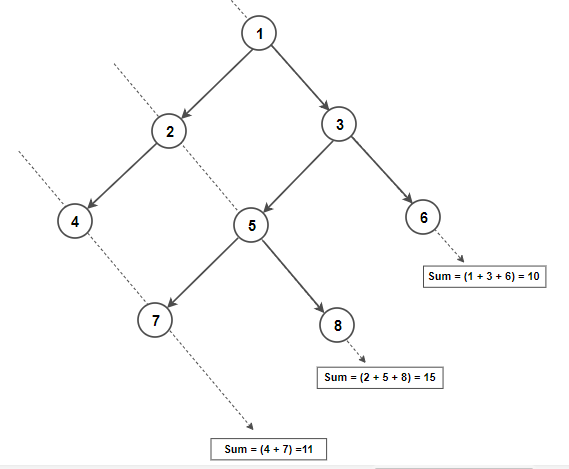
\includegraphics[width=\textwidth]{./Diagonal-Sum-Binary-Tree.png}
        \caption{Suma po dijagonalama stabla}
        \label{fig:slika1}
    \end{minipage}
\end{figure}

\begin{verbatim}
Primer 1:               Primer 2:               Primer 3:               Primer 4:                

Standardni ulaz:        Standardni ulaz:        Standardni ulaz:        Standardni ulaz: 
1                       2                       3                       2 
-5 -5 0 0 3 -8          4 2 1 7 7 9 6           1 1 1 1                 1 -3 -1 4 2 10 3 6 20 8 15

Standardni izlaz:       Standardni izlaz:       Standardni izlaz:       Standardni izlaz:        
-2                      9                       1                       30 
\end{verbatim}  
\end{enumerate}

%------------------------------------------------------------------
\section{Programiranje 2, ispit, septembar1 2019.}
%------------------------------------------------------------------

\begin{enumerate}
\item U datoteci {\tt plate.txt} dat je spisak zarada u različitim gradovima oblika {\tt Grad Plata}. Gradovi se mogu pojaviti više puta. Naziv grada je maksimalne dužine $20$ karaktera. Plata je realan broj (koristiti realne brojeve dvostruke tačnosti za zapis plata). Podatke sortirati rastuće prema nazivu grada, a potom opadajuće prema platama. Kao argument komandne linije zadaje se broj {\tt k} ($k /ge 1$). Ispisati sortirane podatke (naziv grada i plata na tri decimale) tako što se za svaki grad ispiše po {\tt k} plata. Ako neki grad ima manje od {\tt k} plata onda ispisati one plate koje za taj rad postoje i ne prijavljivati grešku. Nije poznato koliko ima podataka u datoteci. Neka korak realokacije bude {\tt 10}. U slučaju greške ispisati {\tt -1} na standardni izlaz za greške.
\begin{verbatim}
Primer 1:                      Primer 2:                   

Pozivanje:  ./a.out 3          Pozivanje: ./a.out 5                   
                                                                                
Datoteka plate.txt:            Datoteka plate.txt:            Standarni izlaz:
Beograd 43400                  Beograd 43400                  Beograd 220300.000
Valjevo 23800.88               Valjevo 23800.88               Beograd 147500.000
Beograd 88232.22               Beograd 88232.22               Beograd 90230.000
Beograd 88232.52               Beograd 88232.52               Beograd 88232.520
Sabac 31200                    Sabac 31200                    Beograd 88232.220
Lazarevac 44500.32             Lazarevac 44500.32             Jagodina 334500.000
Lazarevac 120304.33            Lazarevac 120304.33            Jagodina 44900.200
Valjevo 56200                  Valjevo 56200                  Krusevac 38232.220
Beograd 220300                 Beograd 220300                 Krusevac 33545.450
Lazarevac 76900.23             Lazarevac 76900.23             Lazarevac 120304.330
Beograd 147500                 Beograd 147500                 Lazarevac 76900.230
                               Beograd 90230                  Lazarevac 53290.000
Standarni izlaz:               Valjevo 77820                  Lazarevac 44500.320
Beograd 220300.000             Krusevac 33545.45              Sabac 31200.000
Beograd 147500.000             Jagodina 44900.20              Valjevo 89600.000
Beograd 88232.520              Beograd 78230                  Valjevo 77820.000
Lazarevac 120304.330           Jagodina 334500                Valjevo 56200.000
Lazarevac 76900.230            Krusevac 38232.22              Valjevo 23800.880
Lazarevac 44500.320            Lazarevac 53290
Sabac 31200.000                Valjevo 89600
Valjevo 56200.000
Valjevo 23800.880              

-----------------------------------------------------------
Primer 3:                          Primer 4:

Pozivanje:  ./a.out                Pozivanje: ./a.out -10

Standardni izlaz za greske:        Standardni izlaz za greske:
-1                                 -1
\end{verbatim}

\item Sa standardnog ulaza unosi se ceo broj. Ispisati broj vodećih nula i broj krajnjih nula u binarnom zapisu broja. {\em Napomena: Koristiti tip {\tt int} za čuvanje broja. Prikazani izlaz je u sistemu u kome je {\tt int} $32$ bita.}
\begin{verbatim}
Primer 1:                Primer 2:               Primer 3:                  Primer 4:
Standardni ulaz:         Standardni ulaz:        Standardni ulaz:           Standardni ulaz:
5                        216                     26304                      -10

Standardni izlaz:        Standardni izlaz:       Standardni izlaz:          Standardni izlaz:
29 0                     24 3                    17 6                       0 1
\end{verbatim}

% (zadatak se jednostavno resava sa dva pokazivaca, demonstrirati na tabli)
\item Sa standarnog ulaza unosi se lista celih brojeva. Na, primer, pretpostaviti da je uneta lista {\tt a1 -> a2 -> ... -> an -> b1 -> b2 -> ... -> bn}. Izmeniti listu tako da je novodobijena lista oblika {\tt a1 -> b1 -> a2 -> b2 -> ... -> an -> bn}. Nije dozvoljeno kreiranje nove liste ili novih čvorova. Pretpostaviti da uneta lista ima paran broj elemenata (i ne resavati slucaj kada lista ima neparan broj elemenata). {\em Pomoćna napomena: Zadatak se može rešiti korišćenjem dva pokazivača, jedan ide od početka liste ({\tt a1}), a drugi od sredine ({\tt b1})} {\em Napomena: Za rad sa listama obavezno koristiti datu biblioteku ({\tt liste.c} i {\tt liste.h}). Zadatak se mora rešiti korišćenjem listi, u suprotnom broj osvojenih poena je $0$.}
\begin{verbatim}
Primer 1:                             Primer 2:             

Standardni ulaz:                      Standardni ulaz:      
20 10 -7 17 0 -30                     5  1                   

Standardni izlaz:                     Standardni izlaz:     
[20, 17, 10, 0, -7, -30]              [5, 1]          
---------------------------------------------------------------------------
Primer 3:                             Primer 4:   

Standardni ulaz:                      Standardni ulaz:
-9 -10 8 -200 -400 500                1 2 3 10 20 30

Standardni izlaz:                     Standardni izlaz:
[-9, -200, -10, -400, 8, 500]         [1, 10, 2, 20, 3, 30]
\end{verbatim}

\item Napisati funkciju koja proverava da li je binarno pretraživačko strukturno (tj. binarno uređeno) stablo simetrično (pogledati sliku \ref{fig:slika1}). Funkcija vraća $1$ ako je stablo simetrično, a $0$ inače (strukturno označava da se ne posmatraju vrednosti već samo struktura stabla). Sa standardnog ulaza se učitavaju elementi 3 binarna pretraživačka strukturna (tj. binarna uređena) stabla koji su celi brojevi. Svako stablo se učitava do (\texttt{EOF}). Za svako stablo pozvati napisanu funkciju i ispisati rezultat na standarni izlaz. 
\textit{Napomena: Za rad sa binarnim pretraživačkim stablima obavezno koristiti datu biblioteku (\textbf{stabla.h} i \textbf{stabla.c}). Zadatak se mora rešiti korišćenjem binarnog pretraživačkog stabla i ispis traženih vrednosti mora biti izvršen obilaskom čvorova stabla. U suprotnom broj osvojenih poena je $0$.}

\begin{figure}[h!]
    \centering
    \begin{minipage}[b]{0.50\textwidth}
        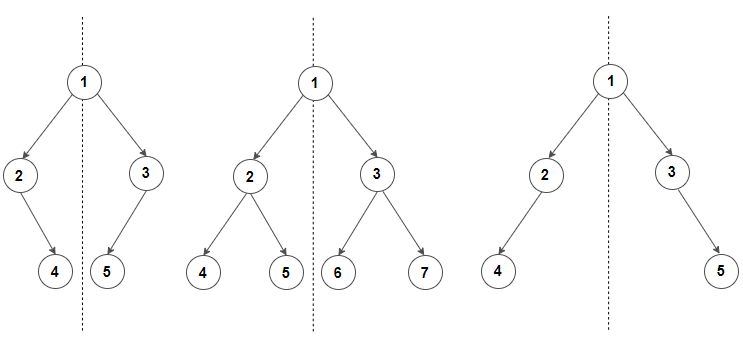
\includegraphics[width=\textwidth]{./Symmetric-Binary-Tree.png}
        \caption{Simetrična stabla}
        \label{fig:slika1}
    \end{minipage}
\end{figure}

\begin{verbatim}
Primer 1:               Primer 2:            Primer 3:            Primer 4:                

Standardni ulaz:        Standardni ulaz:     Standardni ulaz:     Standardni ulaz: 
10 5 15 8 12            10 5 1 15 12                              10 5 15 1 8 12 20 -5 6 13 30
10 5 15 8 12 1 20       10 5 15 20 30 8 1    1 2 -1               10 5 15 1 8 12 20 -5 9 13 30
10 5 15 1 20            10 5 15 1 20         10 5 1 6             10 5 20 8 15 7 18

Standardni izlaz:       Standardni izlaz:    Standardni izlaz:    Standardni izlaz:        
1 1 1                   0 0 1                1 1 0                1 0 1 
\end{verbatim}  
\end{enumerate} 

%--------------------------------------------------------------
\section{Programiranje 2, ispit, septembar2 2019.}
%--------------------------------------------------------------


\begin{enumerate}
\item U datotekama \texttt{dir1.txt} i \texttt{dir2.txt} nalaze se nazivi fajlova koji se nalaze unutar dva direktorijuma \texttt{dir1} i \texttt{dir2}. Nazivi fajlova su sortirani leksikografski rastuće. Potrebno je formirati novi direktorijum \texttt{dir3} koji je unija ova dva direktorijuma, pri čemu nije dozvoljeno da se unutar direktorijuma nalaze dva fajla sa istim nazivom. Ispisati nazive fajlova koji trebaju da se nalaze u novom direktorijumu na standardni izlaz u leksikografski rastućem poretku. Pretpostaviti da je maksimalna dužina naziva fajla 50 karaktera.
\begin{verbatim}
Primer 1:                        Primer 2:                        Primer3:           

dir1.txt:     dir2.txt:          dir1.txt:     dir2.txt:          dat1.txt:     dat2.txt:           
CAS1.pdf      704.pdf            1.c           stabla.c                         1i1a-spisak
CAS2.pdf      718.pdf            a.out         stabla.h                         1i1b-spisak
CAS3.pdf      BIM.pdf            stabla.c      zad                              1i1c-spisak
CAS4.pdf      DLAB.pdf           stabla.h      zad.c                            1i2a-spisak
              JAG1.pdf                                                          1i2b-spisak
              JAG2.pdf                                                          1i2c-spisak
              RLAB.pdf

Standardni izlaz:                Standardni izlaz:                Standardni izlaz:   
704.pdf                          1.c                              1i1a-spisak
718.pdf                          a.out                            1i1b-spisak
BIM.pdf                          stabla.c                         1i1c-spisak
CAS1.pdf                         stabla.h                         1i2a-spisak
CAS2.pdf                         zad                              1i2b-spisak
CAS3.pdf                         zad.c                            1i2c-spisak
CAS4.pdf
DLAB.pdf
JAG1.pdf
JAG2.pdf
RLAB.pdf
\end{verbatim}

\item Napisati rekurzivnu funkciju \texttt{void kvadrati(unsigned a, unsigned b)} koja ispisuje na standardni izlaz sve cele brojeve iz intervala \texttt{[a, b]} koji su kvadrati nekog celog broja. Napisati potom glavni program koji cele brojeve \texttt{a} i \texttt{b} dobija kao argumente komandne linije i poziva funkciju \texttt{kvadrati}. U slučaju greške na standardni izlaz za greške ispisati -1. \emph{Uputstvo}: Napisati odvojenu funkciju koja proverava da li je ceo broj kvadrat nekog celog broja.
\begin{verbatim}
Primer1:                    Primer2:                     Primer3:                    
 
Pozivanje: ./a.out 0 10     Pozivanje: ./a.out 36 36     Pozivanje: ./a.out 36 35    

Standardni izlaz:           Standardni izlaz:            Standardni izlaz:           
1 4 9                       36                           -1                          
\end{verbatim}

% (napomenuti da rezultat nije lista) 
\item Sa standarnog ulaza unosi se lista celih brojeva. Za svaki element liste ispisati koliko puta se taj element u listi pojavljuje. {\em Napomena: Za rad sa listama obavezno koristiti datu biblioteku ({\tt liste.c} i {\tt liste.h}). Zadatak se mora rešiti učitavanjem liste, u suprotnom broj osvojenih poena je $0$. Za čuvanje broja pojavljivanja elemenata korisiti dinamički alociran niz.}
\begin{verbatim}
Primer 1:                             Primer 2:  (primer prazne liste)           

Standardni ulaz:                      Standardni ulaz:      
7 8 10 7 7 20 8 1 8 8 8 8                               

Standardni izlaz:                     Standardni izlaz:     
7: 3
8: 6
10: 1
20: 1
1: 1
---------------------------------------------------------------------------
Primer 3:                             Primer 4:   

Standardni ulaz:                      Standardni ulaz:
-4 -20 -4 -20 1 2 -4 -20 1 2          50 2 20 50 50 0 0 0 0 3 0 0 0 3 0 0 0 5 6

Standardni izlaz:                     Standardni izlaz:
-4: 3                       50: 3
-20: 3                                2: 1
1: 2                                  20: 1
2: 2                                  0: 10
3: 2
5: 1
6: 1
\end{verbatim}

\item Napisati funkciju koja proverava da li je binarno pretraživačko stablo degenerisano u listu. Funkcija vraća $1$ ako je stablo degenerisano u listu, a $0$ inače. Sa standardnog ulaza se učitavaju elementi 3 binarna pretraživačka (tj. binarna uređena) stabla koji su celi brojevi. Svako stablo se učitava do unosa znaka za kraj unosa(\texttt{EOF}). Za svako stablo pozvati napisanu funkciju i ispisati rezultat na standarni izlaz. \textit{Napomena: Za rad sa binarnim pretraživačkim stablima obavezno koristiti datu biblioteku (\textbf{stabla.h} i \textbf{stabla.c}). Zadatak se mora rešiti korišćenjem binarnog pretraživačkog stabla i ispis traženih vrednosti mora biti izvršen obilaskom čvorova stabla. U suprotnom broj osvojenih poena je $0$.}
\begin{verbatim}
         1                     4                   10                        -5      
        /                     /                      \                         \
       1                     3                        11                       -2
      /                     /                           \                     /  \
     1                     1                             12                 -3    0
    /                     / \                              \                / \    \
   1                     0   2                              13            -3  -2    7

Primer 1:               Primer 2:               Primer 3:               Primer 4:                

Standardni ulaz:        Standardni ulaz:        Standardni ulaz:        Standardni ulaz: 
1 1 1 1                 -5 -2 -3 0 -3 -2 7      4 3 2 1 0               10 11 12 12 13
4 3 1 0 2                                       1 1 1 1 1 1 1           -5 -2 0 7
10 11 12 13             10 11 12 13             11 10 12 13             9

Standardni izlaz:       Standardni izlaz:       Standardni izlaz:       Standardni izlaz:        
1 0 1                   0 1 1                   1 1 0                   0 1 1
\end{verbatim}  
 
\end{enumerate} 